\documentclass[conference]{IEEEtran}
\IEEEoverridecommandlockouts

\usepackage{cite}
\usepackage{amsmath,amssymb,amsfonts}
\usepackage{graphicx}
\usepackage{textcomp}
\usepackage{xcolor}
\usepackage{makecell}
\usepackage{listings}
\usepackage{xurl}
\usepackage{hyperref}
\usepackage{booktabs}
\usepackage{float}
\usepackage{tkz-euclide}
\usepackage[citations,hybrid]{markdown}

\definecolor{codegreen}{rgb}{0,0.6,0}
\definecolor{codegray}{rgb}{0.5,0.5,0.5}
\definecolor{codepurple}{rgb}{0.58,0,0.82}
\definecolor{backcolour}{rgb}{0.95,0.95,0.92}

\lstdefinestyle{mystyle}{
    backgroundcolor=\color{backcolour},
    commentstyle=\color{codegreen},
    keywordstyle=\color{magenta},
    numberstyle=\tiny\color{codegray},
    stringstyle=\color{codepurple},
    basicstyle=\ttfamily\footnotesize,
    breakatwhitespace=false,
    breaklines=true,
    captionpos=b,
    keepspaces=true,
    numbers=left,
    numbersep=5pt,
    showspaces=false,
    showstringspaces=false,
    tabsize=2
}
\lstset{style=mystyle}

\markdownSetup{
  renderers = {
    link = {\href{#3}{#1}}
  }
}

\title{UGV-UAV}

\author{
    \IEEEauthorblockN{Jnanesh Sathisha Karmar, Vivek K Kumar, \\
    Dr. G.V.V. Sharma}
    \IEEEauthorblockA{Department of Electrical Engineering, \\Indian Institute of Technology Hyderabad,\\ Kandi, India 502284 \\ gadepall@ee.iith.ac.in}
}

\begin{document}
\maketitle

\begin{abstract}
This work aims to integrate UAV architecture into a UGV platform to develop a unified control system for both domains. This is efficient, and also enables testing of UAVs through UGVs, as effectively UAVs only have an extra dimension.
\end{abstract}

\section{Introduction}

Our goal is to take a drone with a standard multicopter architecture, and try to integrate each component, part by part into a ground vehicle.drone architecture and integrate its core components into a ground-based vehicle. Traditional UAVs rely on high-RPM brushless motors, Electronic Speed Controllers (ESCs), and specialized flight controllers.While components like the power delivery systems and radio transmitters are universally applicable, others—such as the motor control mechanisms—require adaptation for ground use

\bigskip
    \begin{figure}[H]
    \resizebox{0.95\columnwidth}{!}{
    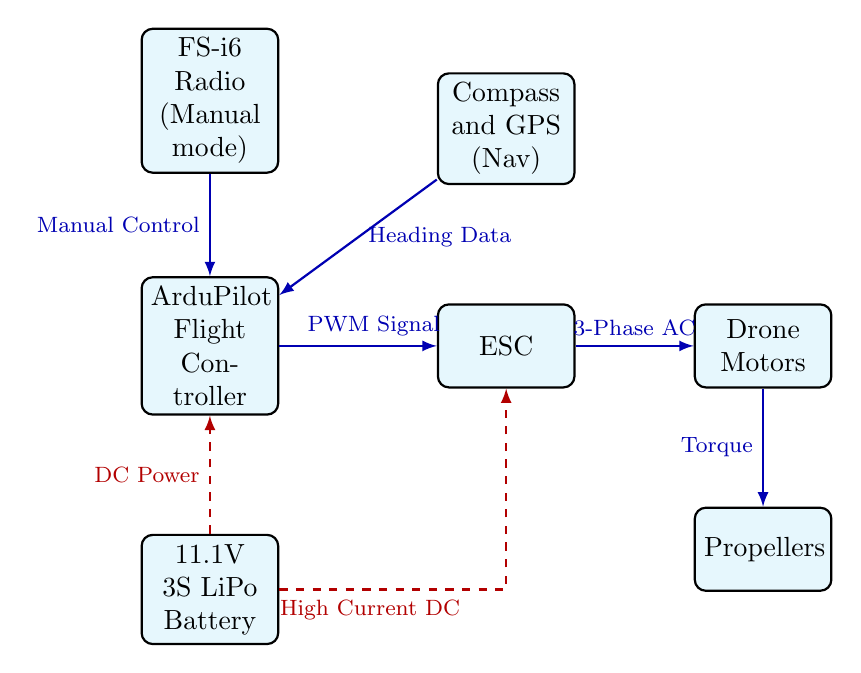
\begin{tikzpicture}[
    node distance=2cm,
    auto,
    block/.style={
        rectangle,
        draw,
        fill=cyan!10,
        text width=1.5cm,
        text centered,
        rounded corners,
        minimum height=3em,
        line width=0.8pt
    },
    line/.style={
        draw,
        -latex,
        thick,
        color=blue!70!black
    },
    power/.style={
        draw,
        -latex,
        dashed,
        thick,
        color=red!70!black
    }
]

    % Components
    \node [block] (fc) {ArduPilot Flight Controller};
    \node [block, right=2cm of fc] (esc) {ESC};
    \node [block, above=1.5cm of esc] (compass) {Compass and GPS (Nav)};
    \node [block, above=1.3cm of fc] (radio) {FS-i6 Radio (Manual mode)};
    \node [block, below=1.5cm of fc] (batt) {11.1V 3S LiPo Battery};
    \node [block, right=1.5cm of esc] (motor) {Drone Motors};
    \node [block, below=1.5cm of motor] (prop) {Propellers};

    % Signal/Data Connections (Blue Solid)
    \path [line] (compass) -- node[pos=0.5, right, font=\footnotesize] {Heading Data} (fc);
    \path [line] (fc) -- node[pos=0.6, above, font=\footnotesize] {PWM Signal} (esc);
    \path [line] (esc) -- node[pos=0.5, above, font=\footnotesize] {3-Phase AC} (motor);
    \path [line] (motor) -- node[pos=0.5, left, font=\footnotesize] {Torque} (prop);
    \path [line] (radio) -- node[pos=0.5, left, font=\footnotesize] {Manual Control} (fc);

    % Power Connections (Red Dashed)
    \path [power] (batt) -- node[pos=0.5, left, font=\footnotesize] {DC Power} (fc);
    \path [power] (batt) -| node[pos=0.2, below, font=\footnotesize] {High Current DC} (esc);
\end{tikzpicture}
}
\caption{Drone architecture}
\label{fig:da}
\end{figure}

The FS-i6 radio system can be reliably used in both the drone framework and the ground vehicle framework. The range of this system is around 500m-1000m in clear air (without obstacles in between).

The same DC power source can be used for both frameworks. The 3S LiPo batteries used in the system are highly versatile.

Due to low torque and high RPM, we concluded that the drone motors cannot directly be used in a ground vehicle framework. Though it might work for certain surfaces, we did not test the effectiveness of this approach. We instead use geared DC Motors (via a motor driver). 
Keeping this in mind, we integrate each of these components into the ground vehicle framework.


\section{Background \& System Components}
\subsection{ArduPilot \& Mission Planner}
ArduPilot\cite{ardupilot} is a versatile autopilot system for multicopters, rovers, boats, and planes. It reads sensors (gyro, GPS)  to controls motors. One of its key advantages is it's ability to handle both high-speed flight stabilization and precise ground steering.This enables the same hardware to be used both as a  flight controller and a ground vehicle controller.


Mission Planner\cite{missionplanner} is a free, open-source Ground Control Station (GCS) software used to configure, monitor, and control autonomous vehicles such as drones, planes, rovers, and boats that run on ArduPilot firmware. It provides a graphical interface to communicate with the flight controller through USB or telemetry radios. Mission Planner allows users to upload flight missions, set waypoints, tune parameters, calibrate sensors, and monitor real-time flight data such as altitude, speed, GPS position, and battery status.
\begin{figure}[H]
    \centering
    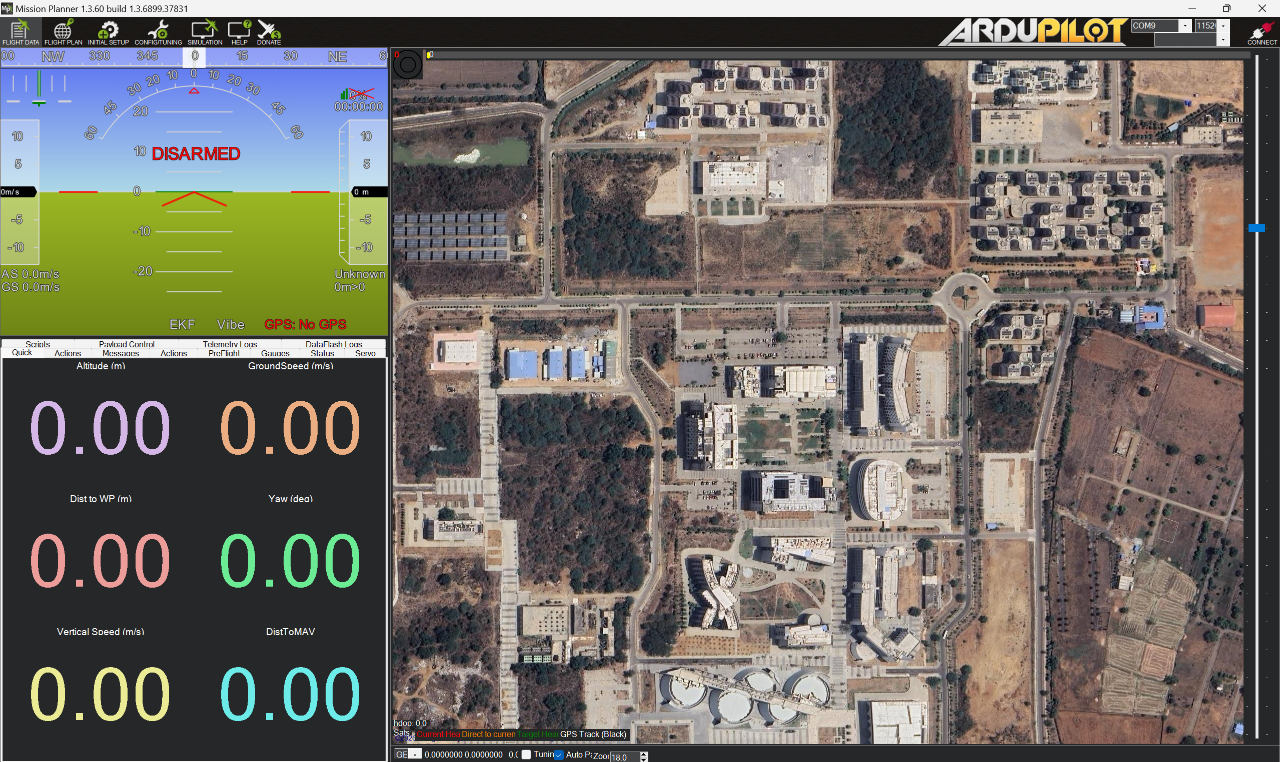
\includegraphics[width=0.8\linewidth]{figs/Mission planner.png}
    \caption{Mission Planner interface}
    \label{fig:placeholder}
\end{figure}
\subsection{Flysky Radio System}
The Flysky FS-i6\cite{flysky} is a 2.4 GHz wireless radio transmitter used for remote control of electronic systems such as drones, robots, RC cars, airplanes, and embedded systems. It is part of the Flysky radio control ecosystem and works together with compatible receivers (such as FS-iA6 or FS-iA6B) to transmit user commands wirelessly to a microcontroller or motor control system.The FS-i6 converts physical inputs from joysticks, switches, and knobs into digital signals, which are transmitted using the AFHDS 2A (Automatic Frequency Hopping Digital System) protocol. The receiver connected to the robot or vehicle interprets these signals and generate corresponding control signals to motors, servos, or microcontrollers.
\begin{figure}[H]
    \centering
    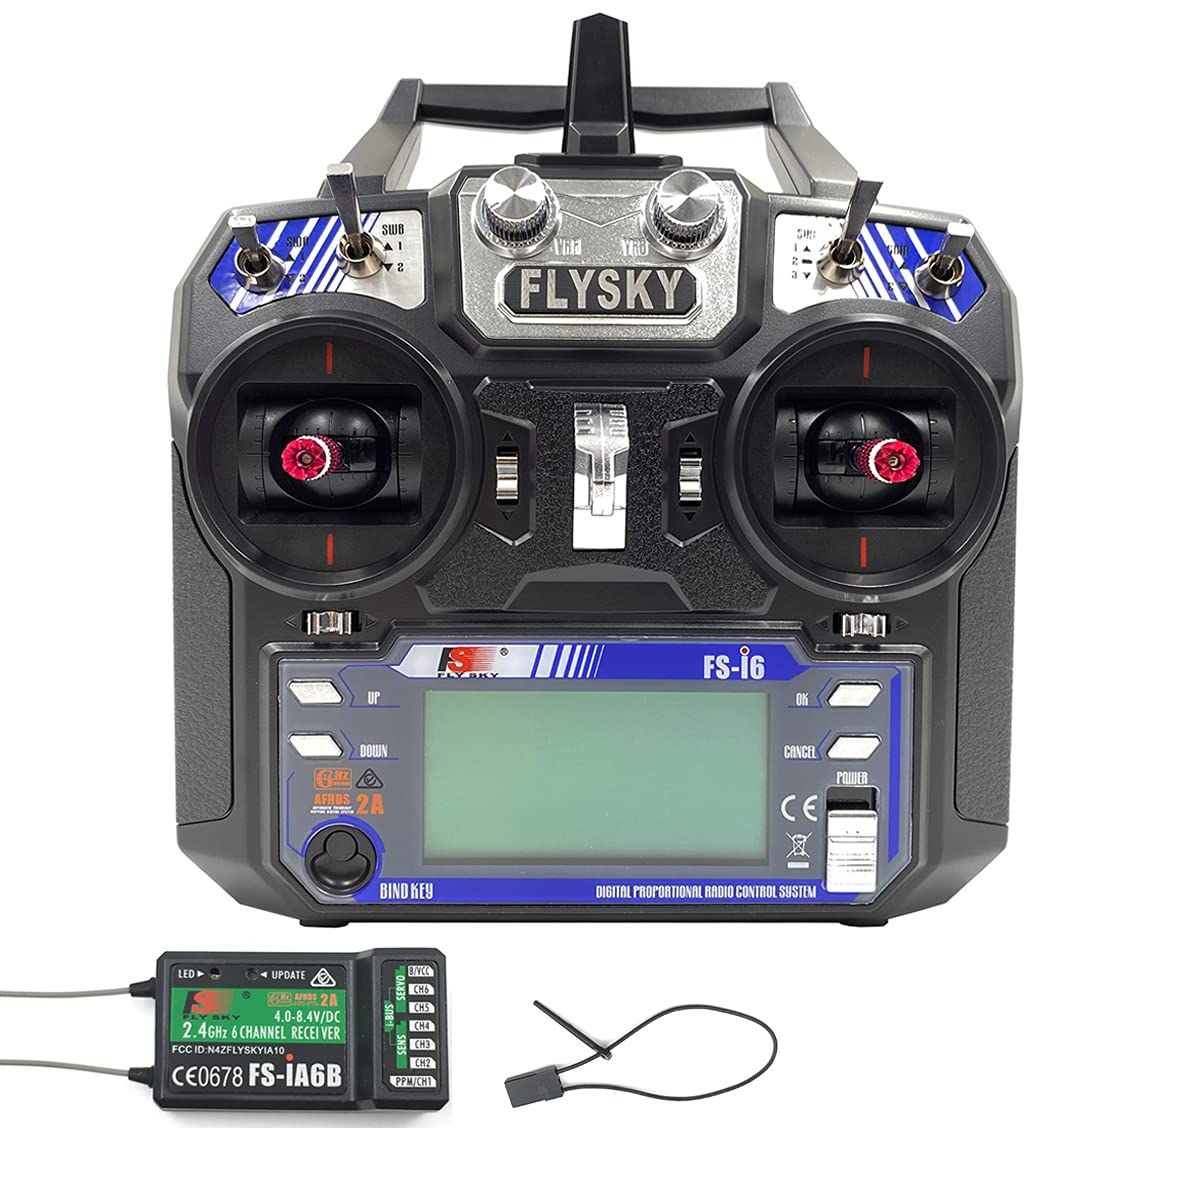
\includegraphics[width=0.9\columnwidth]{figs/flysky.jpg}
    \caption{flysky remote}
    \label{fig:placeholder}
\end{figure}


\section{UAV to UGV Integration}

% \subsection{How to load firmware}
% It is not necessary to write C++ code from scratch to run the microcontroller. Precompiled firmware is available in the \hyperlink{https://ardupilot.org/}{ArduPilot website}, from which Flash specific stacks (e.g., ArduCopter/ArduRover) can be flashed into ArduPilot via Mission Planner.
% Mission Planner can also be used to configure initial parameters(e.g., Radio calibration, ESC calibration) to get the UAV ready for flight.

\subsection{Integration with L298N Motor Drivers}
% \subsection{The Signal Translation Challenge}

\begin{figure}[H]
    \centering
    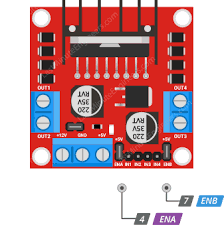
\includegraphics[width=0.4\linewidth]{figs/l298n.png}
    \caption{L298N}
    \label{fig:l298n}
\end{figure}

The system architecture follows a sequential control flow from the APM 2.8 flight controller, through an ESP32 microcontroller, to an L298N motor driver\cite{l298n}, which ultimately powers the DC motors. 
\subsubsection{\textbf{The Signal Translation Challenge}}
A direct connection between the APM and the motor driver is not feasible due to a fundamental signal mismatch. Specifically, the APM 2.8 outputs standard RC servo PWM pulses ranging from 1000~$\mu$s to 2000~$\mu$s, whereas the L298N driver requires logic-level directional inputs (HIGH/LOW) and standard duty-cycle PWM (0--100\%) to regulate speed. 
\subsubsection{\textbf{ESP32 as a Middleware Controller}}
To bridge this gap, the ESP32 functions as a dedicated signal translator. It continuously reads the incoming pulse widths from the APM's throttle and steering outputs and mathematically maps these values to the required motor driver formats. For example, the ESP32 is programmed to interpret a signal of 1000--1450~$\mu$s as a reverse command, 1450--1550~$\mu$s as a neutral deadband for stopping or braking, and 1550--2000~$\mu$s as forward motion. Based on this real-time mapping, the ESP32 drives the appropriate pins on the L298N to achieve precise locomotion.

\subsection{Setup}
\begin{enumerate}
    \item Open Mission Planner and flash the \texttt{ArduRover v2.5.1} firmware onto the APM 2.8 flight controller. Custom C++ code is not required for the APM, as the ArduPilot ecosystem provides precompiled stacks in the \hyperlink{https://ardupilot.org/}{ArduPilot website}.
    \item Calibrate radio, compass, GPS, accelerometer and servo output in Mission Planner
    \item Wire APM 2.8 as follows:
    \begin{itemize}
        \item Inputs: Connect radio receiver and GPS/Compass module. Also power it up through the 5V L298N motor driver line.
        \item Outputs: Connect signal lines of 1 and 3 to ESP32. 
    \end{itemize}
    \item Upload the code into the ESP32 from the following repository
\end{enumerate}
\fbox{\parbox{0.95\columnwidth}{\url{https://github.com/Vivek-Kumar-1907/blob/main/codes/main.ino}
}}

\subsection{Summary Architecture (FlySky)}
\resizebox{0.9\columnwidth}{!}{
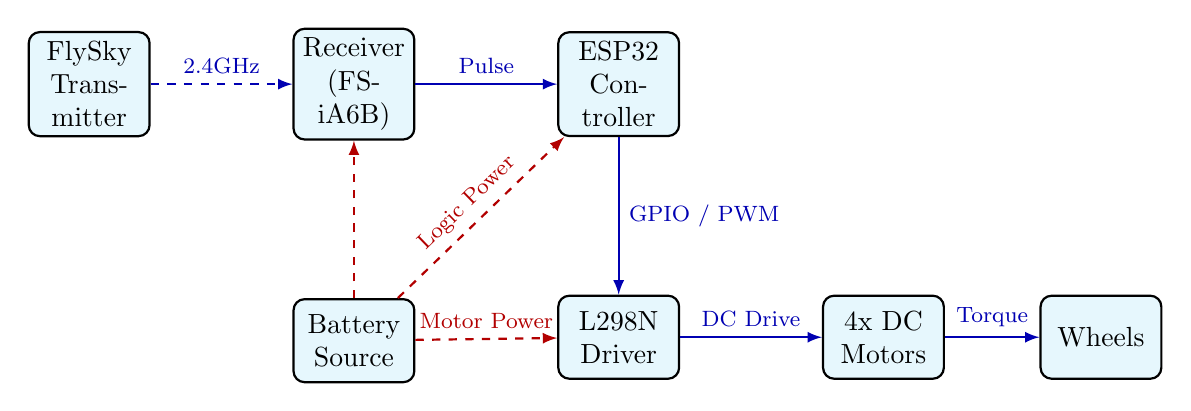
\begin{tikzpicture}[
    node distance=1.5cm and 1.2cm,
    auto,
    block/.style={
        rectangle,
        draw,
        fill=cyan!10,
        text width=1.3cm,
        text centered,
        rounded corners,
        minimum height=3em,
        line width=0.8pt
    },
    line/.style={
        draw,
        -latex,
        thick,
        color=blue!70!black
    },
    wireless/.style={
        draw,
        -latex,
        thick,
        dashed,
        color=blue!70!black
    },
    power/.style={
        draw,
        -latex,
        dashed,
        thick,
        color=red!70!black
    }
]

    % --- Top Row: Control Flow ---
    \node [block] (esp) {ESP32 Controller};
    \node [block, left=1.8cm of esp] (rx) {Receiver (FS-iA6B)};
    \node [block, left=1.8cm of rx] (tx) {FlySky Transmitter};

    % --- Bottom Row: Power & Drive ---
    % Align Driver below ESP32
    \node [block, below=2cm of esp] (driver) {L298N Driver};
    % Align Battery below Receiver
    \node [block, below=2cm of rx] (batt) {Battery Source};
    
    % Motors and Wheels to the right
    \node [block, right=1.8cm of driver] (motor) {4x DC Motors};
    \node [block, right=of motor] (wheel) {Wheels};

    % --- Connections ---

    % 1. Wireless Control (Tx -> Rx)
    \path [wireless] (tx) -- node[above, font=\footnotesize] {2.4GHz} (rx);

    % 2. Receiver Signal (Rx -> ESP32)
    \path [line] (rx) -- node[above, font=\footnotesize] {Pulse} (esp);

    % 3. Motor Control (ESP32 -> Driver)
    \path [line] (esp) -- node[right, font=\footnotesize] {GPIO / PWM} (driver);

    % 4. Power Distribution
    % Battery -> Driver (Motor Power)
    \path [power] (batt) -- node[above, font=\footnotesize] {Motor Power} (driver);
    
    % Battery -> ESP32 (Logic Power) - Path goes Up then Right
    \path [power] (batt) -- node[sloped, above, font=\footnotesize] {Logic Power} (esp);
    
    % Battery -> Receiver (Optional explicit power line, or simplified via ESP)
    % Here we show a small branch for Rx power for completeness
    \path [power] (batt) -- (rx); 

    % 5. Drive Output
    \path [line] (driver) -- node[above, font=\footnotesize] {DC Drive} (motor);
    \path [line] (motor) -- node[above, font=\footnotesize] {Torque} (wheel);

\end{tikzpicture}
}

\subsection{Result}
We have hence successfully translated the entire UAV architecture into an equivalent UGV architecture.


\appendix
\section{Preliminary Testing: Controlling Ground Vehicle with Dabble}

Dabble\cite{dabble} is a mobile application developed by STEMpedia that enables smartphones to function as wireless controllers for microcontroller-based systems such as Arduino, ESP32, and other embedded platforms. It uses Bluetooth communication to connect the smartphone with the hardware, allowing users to control, monitor, and interact with electronic projects in real time.
Dabble provides a set of pre-built modules that simplify interfacing between hardware and smartphone sensors, eliminating the need to design complex mobile applications from scratch. Through its graphical interface, users can access smartphone features such as buttons, sensors, camera input, and motion detection, and transmit that data directly to the microcontroller.

\subsection{Component Architecture with Dabble}
\resizebox{0.95\columnwidth}{!}{%
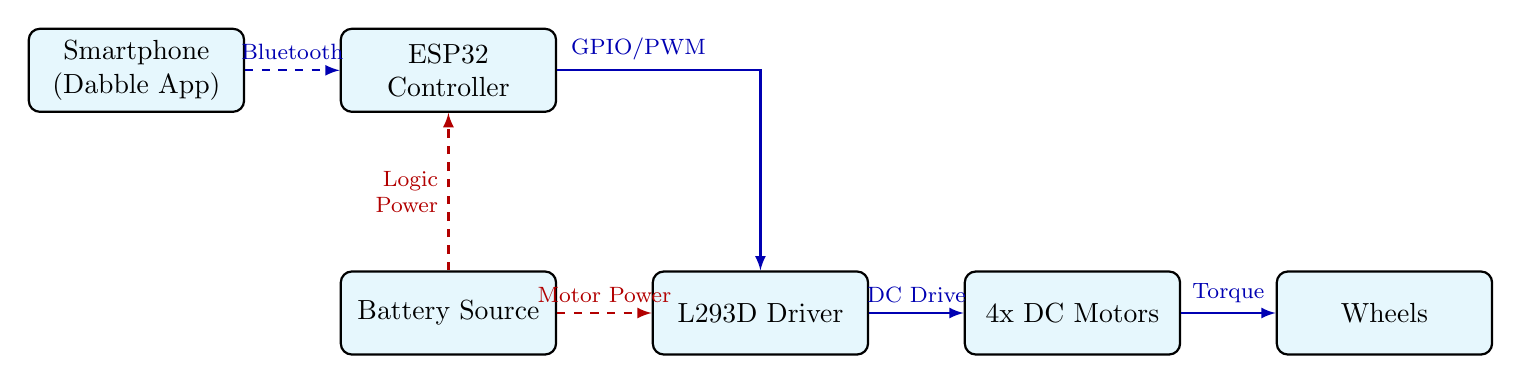
\begin{tikzpicture}[
    node distance=1.2cm and 1.2cm, % Reduced spacing for better fit
    auto,
    block/.style={
        rectangle,
        draw,
        fill=cyan!10,
        text width=2.5cm,
        text centered,
        rounded corners,
        minimum height=3em,
        line width=0.8pt
    },
    line/.style={
        draw,
        -latex,
        thick,
        color=blue!70!black
    },
    wireless/.style={
        draw,
        -latex,
        thick,
        dashed,
        color=blue!70!black
    },
    power/.style={
        draw,
        -latex,
        dashed,
        thick,
        color=red!70!black
    }
]

    % --- Nodes ---
    
    % Top Row
    \node [block] (esp) {ESP32 Controller};
    \node [block, left=of esp] (phone) {Smartphone \\ (Dabble App)};

    % Bottom Row
    % Key Change: Place Battery directly BELOW the ESP32 to simplify wiring
    \node [block, below=2cm of esp] (batt) {Battery Source};
    
    % Place Driver to the RIGHT of Battery
    \node [block, right=of batt] (driver) {L293D Driver};
    
    % Place Motors/Wheels extending to the right
    \node [block, right=of driver] (motor) {4x DC Motors};
    \node [block, right=of motor] (wheel) {Wheels};

    % --- Connections ---
    
    % 1. Bluetooth (Top Left)
    \path [wireless] (phone) -- node[above, font=\footnotesize] {Bluetooth} (esp);

    % 2. Logic Power (Straight Up)
    \path [power] (batt) -- node[left, font=\footnotesize, align=right] {Logic\\Power} (esp);

    % 3. Motor Power (Straight Right)
    \path [power] (batt) -- node[above, font=\footnotesize] {Motor Power} (driver);

    % 4. GPIO/PWM Control (Right then Down)
    % Uses -| to go Horizontal from ESP, then Vertical down to Driver
    \path [line] (esp) -| node[pos=0.2, above, font=\footnotesize] {GPIO/PWM} (driver);

    % 5. Drive & Torque
    \path [line] (driver) -- node[above, font=\footnotesize] {DC Drive} (motor);
    \path [line] (motor) -- node[above, font=\footnotesize] {Torque} (wheel);

\end{tikzpicture}
}

\subsection{Setup and Operation}

\textbf{Setup \& Connection:}
\begin{enumerate}
    \item Install \textbf{Dabble} app (Android).
    \item Enable Bluetooth on your phone.
    \item Open the app and select the \textbf{Gamepad} module.
    \item Tap the \textbf{Plug Icon} (Connect) at the top right.
    \item Select your ESP32 (e.g., \textit{"JNANU"}).
\end{enumerate}

\vspace{0.3cm}
\textbf{Controls:}
\begin{itemize}
    \item Use the \textbf{Digital Mode} (Arrow keys).
    \item \textbf{Up/Down:} Move Forward/Backward.
    \item \textbf{Left/Right:} Turn (Differential Drive).
\end{itemize}

\begin{figure}[H]
\centering
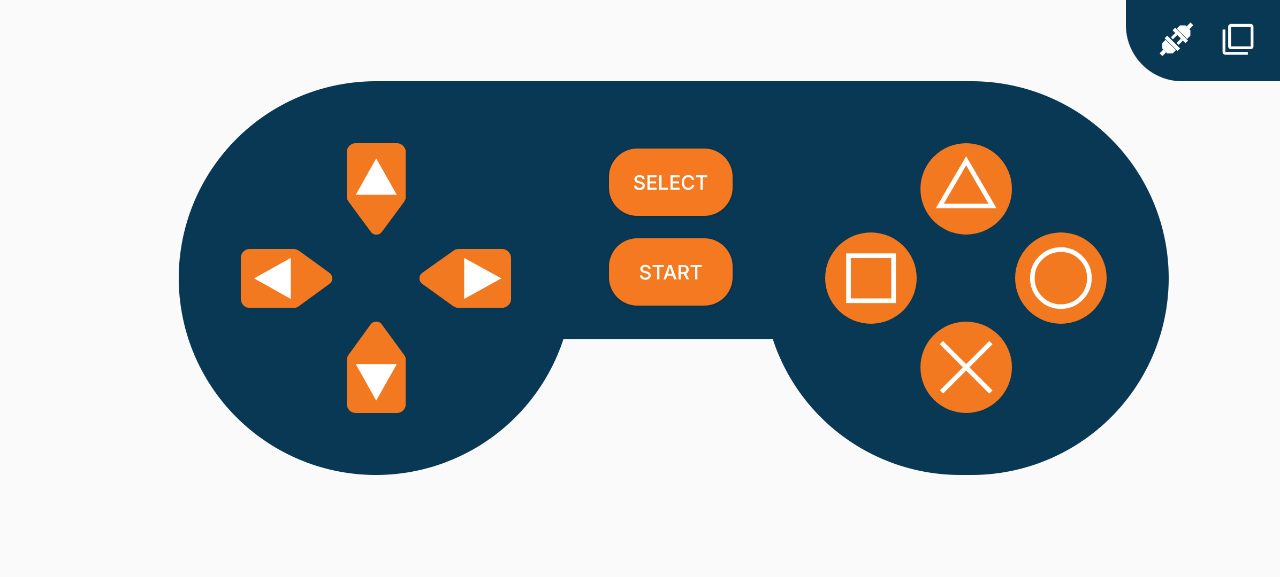
\includegraphics[width=0.9\columnwidth, height=0.8\textheight, keepaspectratio]{figs/dabble.png}
\vspace{0.2cm}
\footnotesize \textit{Dabble Gamepad Interface}
\end{figure}

\bibliographystyle{IEEEtran}
\bibliography{references}

\end{document}
